\documentclass[paper=A4, head_space=20mm, foot_space=20mm, article, jafontsize=12Q, jafontscale=0.92, final]{jlreq} %2 up

\usepackage[no-math]{fontspec}
\usepackage[hiresbb]{graphicx}
\usepackage[dvipsnames]{xcolor}
\usepackage{tikz}
\usepackage[
   unicode,%
   bookmarks=true, %
   bookmarksnumbered=true,%
   pdfusetitle,%
   pdflang=ja-JP, %
   hidelinks%
]{hyperref}
\pagestyle{empty}

\title{SpotScaner v6.1.0}
\author{Kento Yanagisawa}

\begin{document}
   \begin{center}
      \tikzset{
         TargetMarker/.pic={
            \draw[anchor = south west](-0.9, -0.9) node{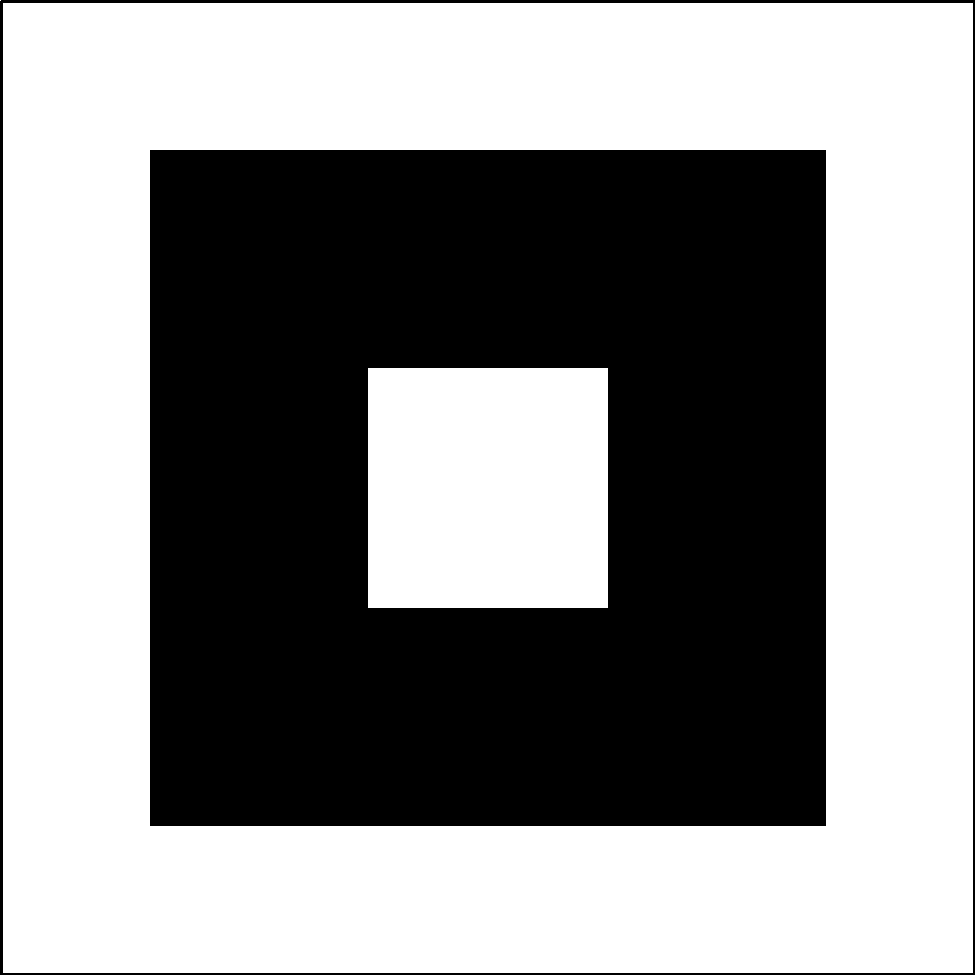
\includegraphics[width = 0.45cm]{marker_image.png}};
         }
      }
      \begin{tikzpicture}[x = 1mm, y = 1mm]
            \filldraw[black](-10, -10) rectangle (137.5, 95);
%%%            \draw[step = 1, lightgray](-10, -10) grid(140, 100);
%%%            \draw[step = 10, gray](-10, -10) grid(140, 100);
            \draw[white](64, 90) node{\fontspec{Monaco}spotscaner --analyze replicator [-t {1,2,3,4,5,6,7,8,9,10}]};
%            \pic at (7.5, 79.5) {TargetMarker};
            \pic at (3.5, 79.5) {TargetMarker};
            \pic at (115.5, 79.5) {TargetMarker};
            \pic at (115.5, -1.5) {TargetMarker};
            \foreach \x in {10, 19, ..., 117} \foreach \y in {10, 19, ..., 73} \draw[line width = 0.5pt, gray](\x, \y) circle(2);
            \draw[white](64, -5) node{\footnotesize\fontspec{Monaco}SpotScaner v6.1.0, Coordinated by Kento Yanagisawa};
      \end{tikzpicture}
   \end{center}
      \vspace{40mm}
   \begin{center}
      \tikzset{
         TargetMarker/.pic={
            \draw[anchor = south west](-1.1, -1.1) node{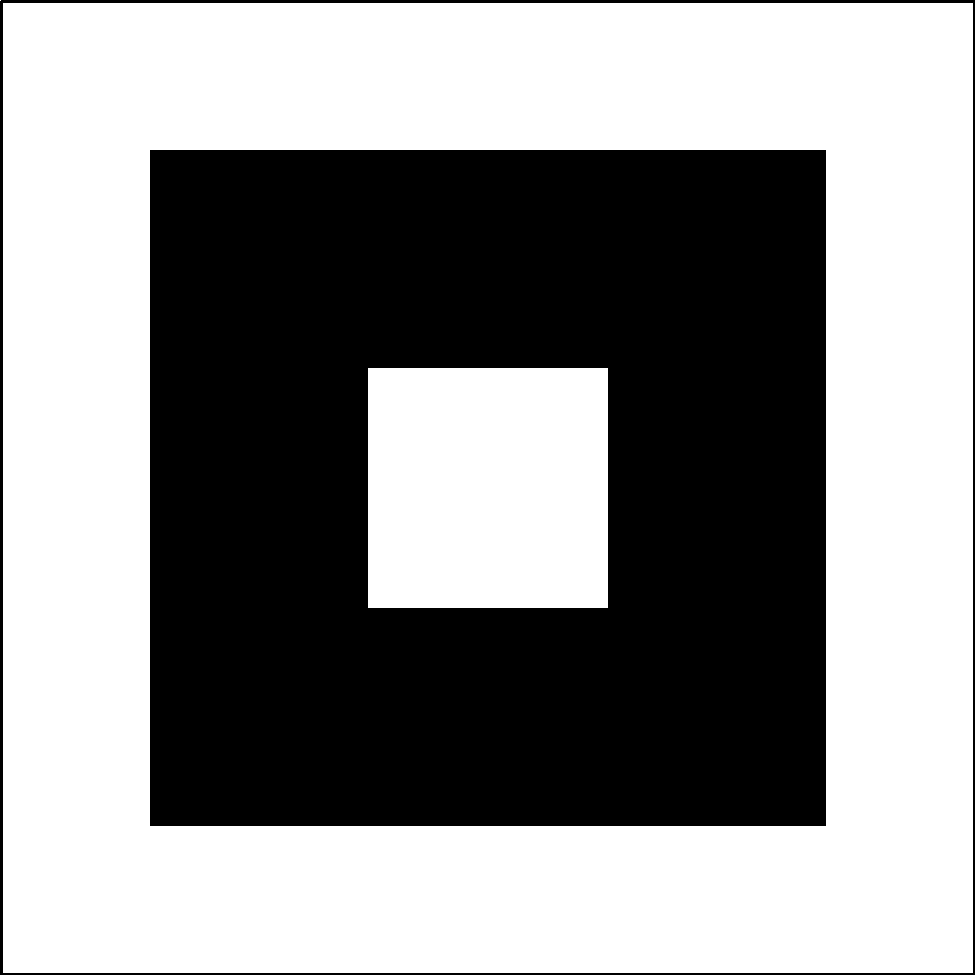
\includegraphics[width = 0.35cm]{marker_image.png}};
         }
      }
      \begin{tikzpicture}[x = 1mm, y = 1mm]
            \filldraw[black](-10, -10) rectangle (137.5, 95);
%            \draw[step = 1, lightgray](-10, -10) grid(140, 100);
%            \draw[step = 10, gray](-10, -10) grid(140, 100);
%            \draw[step = 9.6, blue, shift={(21.81, -0.2)}](0, 0) grid(86.4, 86.4);
            \draw[white](64, 90) node{\fontspec{Monaco}spotscaner --analyze pipette [-t {1,2,3,4,5,6,7,8,9,10}]};
%            \pic at (7.5, 79.5) {TargetMarker};
            \pic[scale = 0.8] at (35.5, 64) {TargetMarker};
            \pic[scale = 0.8] at (94.5, 64) {TargetMarker};
            \pic[scale = 0.8] at (94.5, 19) {TargetMarker};
            \foreach \x in {41.012, 50.612, ..., 98} \foreach \y in {28.6, 38.2, ..., 60} \draw[line width = 0.5pt, gray](\x, \y-1.5) --(\x, \y+1.5);
            \foreach \x in {41.012, 50.612, ..., 98} \foreach \y in {28.6, 38.2, ..., 60} \draw[line width = 0.5pt, gray](\x-1.5, \y) --(\x+1.5, \y);
            \draw[line width = 1pt, white](65, 43) circle(44);
            \draw[white](64, -5) node{\footnotesize\fontspec{Monaco}SpotScaner v6.1.0, Coordinated by Kento Yanagisawa};
      \end{tikzpicture}
   \end{center}
\end{document}